\documentclass[conference]{IEEEtran}

\usepackage[utf8]{inputenc}
\usepackage[T1]{fontenc}
\usepackage[english]{babel}
\usepackage{graphicx}
\graphicspath{{main_ASADA_images/}{Tecnologia_en_Marcha/main_ASADA_images/}}
\usepackage{array}
\usepackage{tabularx}
\usepackage{booktabs}
\usepackage{url}
\usepackage{cite}
\usepackage{tikz}
\usetikzlibrary{arrows.meta,positioning}

\urlstyle{same}
\sloppy

\title{Digitalization of Community-Managed Rural Aqueducts in Costa Rica:\\ An Evidence-Calibrated Synthesis of Three Prototype Developments}

\author{
\IEEEauthorblockN{María José Angulo Campos}
\IEEEauthorblockA{
\textit{Tecnológico de Costa Rica}\\
Cartago, Costa Rica \\
https://orcid.org/0009-0005-5842-1101}
\and
\IEEEauthorblockN{Carlos Montoya Marín}
\IEEEauthorblockA{
\textit{Tecnológico de Costa Rica}\\
Cartago, Costa Rica \\
https://orcid.org/0009-0001-1561-9768}
\and
\IEEEauthorblockN{Juan José Montero-Jiménez}
\IEEEauthorblockA{
\textit{Tecnológico de Costa Rica}\\
Cartago, Costa Rica \\
https://orcid.org/0000-0002-3215-3736}
\and
\IEEEauthorblockN{Juan José Rojas-Hernández}
\IEEEauthorblockA{
\textit{Tecnológico de Costa Rica}\\
Cartago, Costa Rica \\
https://orcid.org/0000-0002-3261-5005}
}

\begin{document}
\maketitle

\begin{abstract}
This article presents a retrospective multiple-case synthesis of three digital-monitoring prototypes developed with community-managed rural aqueducts (ASADAS) in Costa Rica: Las Juntas de Abangares, Playa Sámara, and Paso Ancho--Boquerón. The study asks which operational needs and logical functions recur across the cases, how site constraints alter their physical implementation, and what evidence supports transfer to future deployments. A predefined extraction frame was applied to technical reports, graduation projects, and versioned design artifacts. Evidence was classified from planned work (E0) to sustained field operation (E4) to avoid treating calculations, bench tests, and limited field checks as equivalent. The synthesis identifies a reusable functional chain---measurement, local acquisition and validation, communication, data services, and operator information---with energy, security, health monitoring, and maintainability as cross-cutting concerns. A configurable reference architecture and site-to-module decision criteria make explicit which functions remain stable and which components must change with instrumentation, power, coverage, distance, and maintenance capacity. The cases support functional feasibility for selected subsystems, but none provides E4 evidence. Accordingly, the architecture is a traceable design hypothesis rather than a field-validated universal solution; availability, energy autonomy, alert performance, operator acceptance, costs, and effects on water losses or service continuity require sustained deployment.
\end{abstract}

\begin{IEEEkeywords}
community-managed water systems, rural aqueducts, ASADA, Internet of Things, remote monitoring, MBSE, modular architecture, case synthesis
\end{IEEEkeywords}

\section{Introduction}

Digital transformation in water infrastructure combines sensing, communications, data management, and automation within an operational system \cite{arnell2023making,zulkifli2022iot,velayudhan2022iot}. In resource-constrained settings, remote monitoring can reduce information delays, but successful operation depends on more than connecting a sensor to a cloud service. Retrofit compatibility, energy autonomy, intermittent connectivity, maintainability, and the ability of operators to act on the information are equally important. Prior studies have demonstrated remote monitoring of rural handpumps and solar-powered retrofit nodes \cite{thomson2012gsm,bawankar2024iot}; however, the transfer of such solutions remains contingent on local infrastructure and service arrangements.

Costa Rica has more than 2000 community water organizations, known as ASADAS, that manage local drinking-water systems \cite{direccion2025asadas}. Previous studies have documented limitations in infrastructure condition, maintenance, and technical capacity in rural suppliers \cite{soto2016situacion,gaviria2020risk}. Within this context, Laboratorio Delta at Tecnológico de Costa Rica participated in a sequence of prototypes that progressed from autonomous tank-level acquisition to distributed meter integration and industrial interfaces \cite{chavarria2021implementacion,solorzano2021sistema,oviedo2024desarrollo}. A related ISSE 2025 paper formalized a generic architecture for rural-aqueduct IoT systems using ARCADIA and model-based systems engineering (MBSE) \cite{arguedas2025towards}.

The present article does not claim another field validation of that architecture. Its distinct contribution is an evidence-calibrated reconstruction of the three preceding developments. In contrast with \cite{arguedas2025towards}, which presents the generic MBSE architecture, this study: (i) includes Las Juntas de Abangares; (ii) applies one comparative extraction frame to all three cases; (iii) separates planned, simulated, bench-tested, field-tested, and sustained functions; and (iv) converts the cross-case findings into explicit configuration and verification criteria. The analysis addresses three research questions:

\begin{description}
\item[RQ1:] Which operational needs and logical functions recur across the three developments?
\item[RQ2:] How do site constraints change the physical implementation while the functional chain remains stable?
\item[RQ3:] What level of evidence supports each capability, and what must be verified before transfer to another ASADA?
\end{description}

This framing deliberately limits inference to the documented cases. ``Recurring'' means observed in at least two cases; it does not mean universal among Costa Rican ASADAS. Likewise, ``transferability'' denotes explicit conditions for adaptation and evaluation, not demonstrated performance at an unstudied site.

\section{Method}

\subsection{Study Design and Case Boundaries}

We conducted a retrospective multiple-case synthesis following the logic of bounded case-study comparison \cite{yin2018case}. The unit of analysis was one documented digital-monitoring development associated with a Costa Rican ASADA. The cases were selected purposively because they form a traceable development sequence from the same laboratory and jointly cover: (a) autonomous tank-level monitoring, (b) distributed monitoring using existing meters, and (c) industrial analog and digital interfaces. The available sample is therefore analytically useful but neither random nor representative of all ASADAS.

The primary sources were the final graduation projects and technical reports for Las Juntas de Abangares, Playa Sámara, and Paso Ancho--Boquerón \cite{chavarria2021implementacion,solorzano2021sistema,oviedo2024desarrollo}. Two complementary sources had narrower roles. The ISSE 2025 paper supplied the MBSE separation between operational needs, logical functions, and physical components \cite{arguedas2025towards}. A versioned 2026 repository supplied the status of the current Paso Ancho implementation \cite{deltalabo2026repo}. Because that repository represents a later design iteration, it is reported separately and is not counted as a fourth validated case.

\subsection{Extraction and Cross-Case Analysis}

The same extraction frame was applied to each case:
\begin{enumerate}
\item Context and requirements: operational problem, users, assets, sampling needs, environmental constraints, power, and connectivity.
\item Engineering process: functional decomposition, alternatives, selection criteria, integration steps, test-driven revisions, and unresolved interfaces.
\item Implementation: variables, sensors, controllers, protocols, energy supply, data services, alarms, and control-oriented functions.
\item Evidence: test setting, reference measurement, reported result, supported function, and pending verification.
\end{enumerate}
Details absent from a source were marked unreported rather than inferred. The analysis first summarized each case and then compared coded fields across cases. A need was marked cross-case recurrent when the same operational purpose occurred in at least two developments. Site-specific requirements were retained as constraints. Logical functions were then mapped to physical alternatives without treating a component used once as universally preferable.

No inter-coder reliability statistic was calculated; this is a limitation of the retrospective synthesis. To make the interpretation auditable, the manuscript cites source sections, separates the later repository from the three cases, and provides an evidence and traceability matrix in Table~\ref{tab:evidence}.

\subsection{Evidence Calibration}

To prevent unlike tests from being interpreted as equivalent, each reported capability was assigned the highest level supported by its source:
\begin{itemize}
\item E0: requirement, design, or planned verification only;
\item E1: calculation or simulation;
\item E2: component or bench test;
\item E3: limited field or partial end-to-end test;
\item E4: sustained field operation with defined duration and performance metrics.
\end{itemize}
The scale describes strength of evidence, not technology readiness in general. No new measurements, interviews, prolonged trials, or statistical analyses were performed for this article.

\section{Case Evidence}

\subsection{Las Juntas de Abangares}

CIEDES required tank-level records for water-balance, demand, and supply-capacity studies. Level had been measured approximately every fifteen days and recorded manually. Requirements included time-stamped measurements every hour or every 20 minutes, remote queries, plots, downloads, and off-grid operation \cite[Secs.~4.1--4.3]{chavarria2021implementacion}.

The design compared HTTP and MQTT arrangements and alternatives for sensing, control, and power. HTTP was selected for simple integration at the required frequency. SIM900 connection delays and command failures motivated replacement by a SIM7600 modem, while timed power switching reduced consumption \cite[Secs.~4.4--5.1]{chavarria2021implementacion}. The prototype integrated an AJ-SR04 ultrasonic sensor, Arduino Nano, real-time clock, cellular modem, web database, and solar supply. Tape-measure comparisons supported sensor calibration; functional tests supported transmission, storage, query, plotting, and download. Energy autonomy was supported by sizing calculations and photovoltaic simulation rather than sustained field observation.

\subsection{Playa Sámara}

This case sought distributed hydraulic information and pumping coordination while preserving ARAD Octave meters. Constraints included dispersed assets, off-grid operation, humidity, corrosion, and a reporting interval refined to accommodate the selected MQTT service \cite[Secs.~1.3--2.1]{solorzano2021sistema}. The design separated communication, measurement, and control-oriented functions. Meter tests led to revisions in pulse interpretation and resolution before final checks.

Three ESP32-based devices acquired Octave SSR pulses and combined solar power, LoRa links, a gateway, MQTT, and Adafruit IO. The report uses LoRaWAN terminology; the available description directly supports LoRa links with a gateway and application packets. Display-referenced comparisons produced 0\% difference in accumulated volume and 0.72\% or 0.73\% difference in average flow, depending on the report section \cite[Sec.~5.2.2 and conclusions]{solorzano2021sistema}. This internal discrepancy, the absence of absolute reference accuracy, and the uninstalled pumping modification limit the claim to tested acquisition and communication functions.

\subsection{Paso Ancho--Boquerón (2024)}

Difficult tank access motivated remote level, flow, and volume monitoring while preserving compatible Octave meters. Requirements separated node architecture, measurement integration, gateway integration, and visualization \cite[Secs.~1.3--2.1]{oviedo2024desarrollo}. An M-Duino 21+LoRa acquired a conditioned 4--20~mA level signal and Octave registers through Modbus. Solar power supplied the node; LoRa connected it to a gateway, and WiFi connected the gateway to ThingSpeak.

Field checks supported Modbus acquisition. Later integration at TEC used a representative tank for level and node-to-gateway communication. Because a compatible Octave meter was unavailable there, the end-to-end visualization used earlier field readings and assumed flow and volume values \cite[Sec.~6.2 and Annexes~9.2--9.3]{oviedo2024desarrollo}. The evidence therefore supports partial integration, not sustained operation of the complete chain.

\begin{table*}[t]
\caption{Evidence and traceability across the three cases.}
\label{tab:evidence}
\centering
\scriptsize
\renewcommand{\arraystretch}{1.12}
\begin{tabularx}{\textwidth}{@{}>{\raggedright\arraybackslash}p{0.14\textwidth}>{\raggedright\arraybackslash}X>{\raggedright\arraybackslash}p{0.12\textwidth}>{\raggedright\arraybackslash}X>{\raggedright\arraybackslash}X@{}}
\toprule
\textbf{Case and source} & \textbf{Highest supported evidence} & \textbf{Level} & \textbf{Supported functions} & \textbf{Principal limit for synthesis} \\
\midrule
Las Juntas \cite{chavarria2021implementacion} & Calibration, functional web-chain checks, and power-hardware checks; energy sizing and simulation & E3 for limited functions; E1 for autonomy & Level acquisition, cellular HTTP, storage, query, plots, downloads & Duration, field availability, and long-term energy autonomy unreported \\
Playa Sámara \cite{solorzano2021sistema} & Bench and limited field checks of meter interface, firmware, radio link, and data service & E3 & Pulse acquisition, LoRa/gateway path, MQTT service, alarm logic & Display-referenced comparison; flow discrepancy; actuation uninstalled; no sustained record \\
Paso Ancho--Boquerón \cite{oviedo2024desarrollo} & Field Modbus check and partial integration at TEC & E3 & 4--20~mA input, Modbus acquisition, LoRa reception, cloud demonstration & Representative or assumed values used in integration; no sustained end-to-end operation \\
\bottomrule
\end{tabularx}
\end{table*}

\section{Cross-Case Findings}

\subsection{Recurring Needs and Stable Functions}

Five operational needs recurred. First, remote observability replaced intermittent manual records with time-stamped data. Second, interoperability preserved useful assets through ultrasonic, pulse, analog, or Modbus interfaces. Third, off-grid operation required selectable energy and communication arrangements. Fourth, data had to be transformed into accessible plots, downloads, alarms, or control-oriented information. Fifth, reliability and maintainability required explicit calibration, interface checks, system health, recovery, and documented configuration.

Across the three cases, these needs map to a stable logical chain:
\begin{center}
\small measurement $\rightarrow$ acquisition and local validation $\rightarrow$ communication\\
$\rightarrow$ storage and processing $\rightarrow$ operator information.
\end{center}

The chain is more stable than any physical component. For example, HTTP can be replaced by MQTT, LoRa by cellular communication, and an ultrasonic sensor by 4--20~mA or Modbus without changing the purpose of the corresponding logical function.

\subsection{Reference Architecture}

Figure~\ref{fig:architecture} converts the comparison into a configurable reference architecture. Solid arrows show the required measurement-to-information path. The upper band contains site constraints that determine physical choices. The lower band contains cross-cutting requirements that must be verified across modules. The architecture is therefore not a bill of materials: it is a set of stable functions, controlled interfaces, and selectable implementations.

\begin{figure*}[t]
\centering
\resizebox{0.96\textwidth}{!}{%
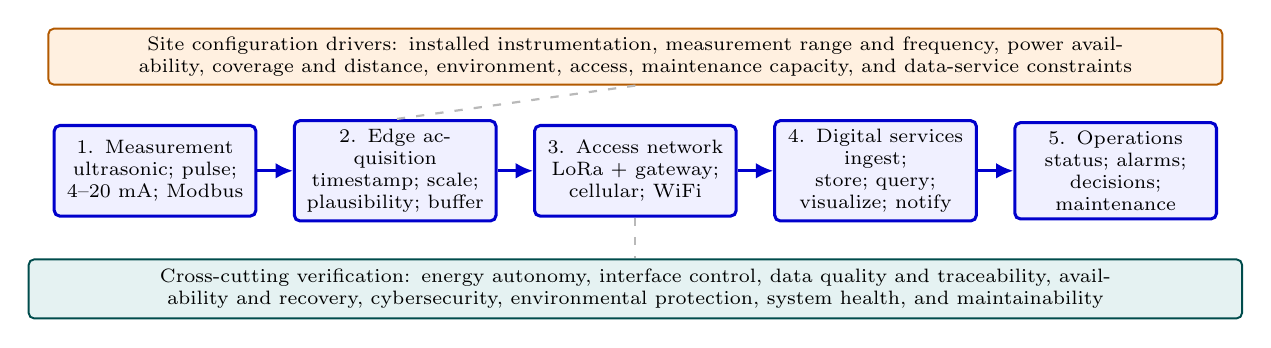
\begin{tikzpicture}[
font=\scriptsize,
process/.style={draw=blue!80!black, line width=1.1pt, rounded corners=2pt, fill=blue!6, align=center, minimum height=1.15cm, text width=2.35cm, inner sep=3pt},
topband/.style={draw=orange!70!black, line width=0.7pt, rounded corners=2pt, fill=orange!12, align=center, minimum height=0.65cm, text width=14.7cm, inner sep=3pt},
bottomband/.style={draw=teal!60!black, line width=0.7pt, rounded corners=2pt, fill=teal!10, align=center, minimum height=0.75cm, text width=15.2cm, inner sep=3pt},
arrow/.style={-{Latex[length=2.2mm,width=2mm]}, draw=blue!80!black, line width=1pt}
]
\node[topband] (top) at (0,2.0) {Site configuration drivers: installed instrumentation, measurement range and frequency, power avail-\\ability, coverage and distance, environment, access, maintenance capacity, and data-service constraints};

\node[process] (m) at (-6.1,0.55) {1. Measurement\\ultrasonic; pulse;\\4--20~mA; Modbus};
\node[process] (e) at (-3.05,0.55) {2. Edge acquisition\\timestamp; scale;\\plausibility; buffer};
\node[process] (n) at (0,0.55) {3. Access network\\LoRa + gateway;\\cellular; WiFi};
\node[process] (d) at (3.05,0.55) {4. Digital services\\ingest; store; query;\\visualize; notify};
\node[process] (o) at (6.1,0.55) {5. Operations\\status; alarms;\\decisions; maintenance};

\draw[arrow] (m.east) -- (e.west);
\draw[arrow] (e.east) -- (n.west);
\draw[arrow] (n.east) -- (d.west);
\draw[arrow] (d.east) -- (o.west);

\node[bottomband] (bottom) at (0,-0.95) {Cross-cutting verification: energy autonomy, interface control, data quality and traceability, avail-\\ability and recovery, cybersecurity, environmental protection, system health, and maintainability};

\draw[gray!55, line width=0.8pt, dash pattern=on 3pt off 4pt] (top.south) -- (e.north);
\draw[gray!55, line width=0.8pt, dash pattern=on 3pt off 4pt] (n.south) -- (bottom.north);
\end{tikzpicture}}
\caption{Evidence-derived configurable reference architecture. Logical functions remain stable; physical implementations are selected from site constraints and verified end to end.}
\label{fig:architecture}
\end{figure*}

\subsection{Configuration and Verification Criteria}

Table~\ref{tab:criteria} operationalizes transferability. It does not prescribe one technology; instead, it identifies the minimum decision evidence required before replication. A module is transferable only if its interface, site assumptions, and acceptance criteria are documented.

\begin{table*}[t]
\caption{Site-to-module decision and verification criteria.}
\label{tab:criteria}
\centering
\scriptsize
\renewcommand{\arraystretch}{1.12}
\begin{tabularx}{\textwidth}{@{}>{\raggedright\arraybackslash}p{0.20\textwidth}>{\raggedright\arraybackslash}p{0.22\textwidth}>{\raggedright\arraybackslash}X>{\raggedright\arraybackslash}X@{}}
\toprule
\textbf{Observed site condition} & \textbf{Configuration decision} & \textbf{Required specification} & \textbf{Minimum verification before deployment} \\
\midrule
Existing compatible meter or industrial sensor & Preserve asset; select pulse, 4--20~mA, or Modbus interface & Register/pulse definition, range, scaling, isolation, wiring, error handling & Compare against a traceable reference over the operating range; verify disconnect, invalid-value, and recovery behavior \\
No fixed power & Solar/battery node with duty cycling & Load profile, sampling/transmission interval, autonomy target, solar resource, enclosure & Bench load test plus energy balance; then observe battery and node availability under representative weather \\
Dispersed nodes with gateway access & LoRa-based local link & Distance, terrain, payload, reporting interval, packet policy, gateway power/backhaul & Site survey and packet-delivery test at each location; verify buffering and recovery after link loss \\
Cellular coverage without local Internet & Direct cellular node & Operator/bands, signal range, data plan, retry policy, consumption & Coverage test across expected conditions; end-to-end upload, retry, buffer, and power-cycle recovery \\
Operator needs alarms or control & Add notification first; introduce actuation only after monitoring is reliable & Threshold owner, response workflow, fail-safe state, authorization, audit trail & Alarm precision and delivery-time test; control hazard analysis and supervised acceptance test before actuation \\
\bottomrule
\end{tabularx}
\end{table*}

\section{Current Paso Ancho Iteration}

The current Paso Ancho application is a later instantiation under development and is not evidence of completed deployment \cite{deltalabo2026repo}. Its mission documentation includes mobile monitoring, overflow and insufficient-supply alerts, Octave and level-sensor acquisition, operation without fixed power or Internet, environmental protection, maintainability, availability, and cybersecurity.

The reviewed version initializes RS-485, reads flow and volume through Modbus, scales an analog height input to 0--5~m, and emits results through a serial port. The SIM7600 wrapper is commented out, so LTE transmission, remote upload, and end-to-end integration remain at E0. The documented 24~V One-Wire depth sensor also differs from the analog interface implemented in firmware. Before deployment, the team should issue an interface control document that reconciles the physical sensor, electrical conversion, firmware input, engineering units, range, resolution, fault values, and calibration procedure.

Planned tests should cover the full path in Fig.~\ref{fig:architecture}, including local validation, transfer without fixed Internet, storage, visualization, notifications, node health, recovery, access control, and backup. Performance claims will require the deployed firmware and configuration, raw data, test protocols, defined acceptance criteria, and observation duration.

\section{Discussion}

\subsection{What Transfers and What Does Not}

The cases support transfer of logical functions more strongly than transfer of components. Remote observability, time-stamped acquisition, an end-to-end communication path, persistent data, operator access, and maintainability are common purposes. Sensor type, protocol, power arrangement, controller, gateway, and cloud service are site-dependent choices. This distinction is the principal value of the MBSE lens: operational needs and logical behavior can be retained while physical implementations vary \cite{arguedas2025towards,voirin2018arcadia}.

Incremental modernization can preserve Octave meters and other useful assets, reducing replacement and disruption. The trade-off is additional complexity in signal conditioning, register or pulse interpretation, version control, calibration, and fault diagnosis. Likewise, LoRa can reduce wide-area node energy consumption when a maintainable gateway and backhaul are available, whereas cellular communication can remove the gateway but increase node consumption, service dependence, and recurring cost. The present evidence does not establish a universally superior option.

The prototypes also show why monitoring, decision logic, and actuation should be verified separately. Data acquisition may be functional while alarms, operational response, or pumping control remain untested. Introducing control before the monitoring chain has demonstrated reliable timestamps, units, fault handling, availability, and recovery would convert data-quality failures into operational hazards.

\begin{figure}[t]
\centering
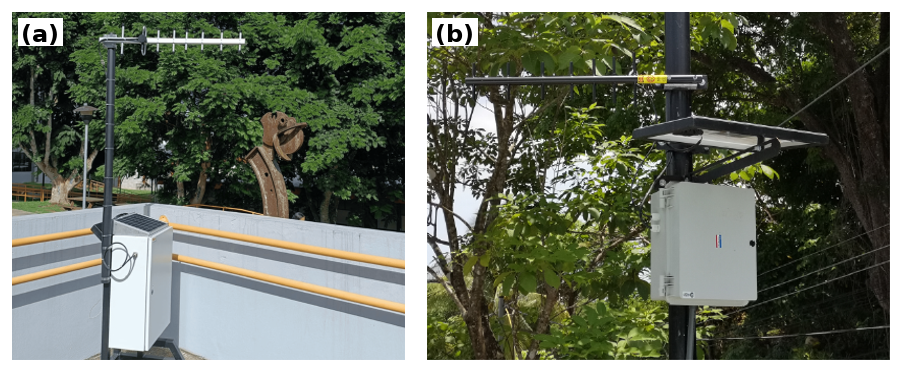
\includegraphics[width=\columnwidth]{figure-000.png}
\caption{Representative documented hardware: (a) Paso Ancho--Boquerón and (b) Playa Sámara \cite{solorzano2021sistema,oviedo2024desarrollo}. The photographs illustrate physical variability rather than an invariant architecture.}
\label{fig:hardware}
\end{figure}

\subsection{Evidence Limits and Threats to Validity}

The synthesis has four principal limitations. First, all cases originated from one institutional development line; shared personnel and design preferences reduce independence. Second, source reports differ in purpose, terminology, test conditions, and level of detail. Third, several comparisons use equipment displays, simulations, representative inputs, or assumed values rather than traceable reference instruments and sustained end-to-end data. Fourth, the retrospective coding was not independently replicated and no stakeholder interviews were conducted for this article.

Consequently, the findings support a design framework and functional feasibility under reported test conditions, not population-level generalization. No analyzed source establishes sustained availability, long-term energy autonomy, maintenance burden, cybersecurity performance, operator acceptance, cost effectiveness, reduced water loss, or improved service continuity. The proposed criteria strengthen analytical transferability, but empirical transfer remains to be tested at an additional site.

\section{Operational Evaluation Agenda}

The next deployment should use a preregistered verification matrix linking every requirement to an interface, test, acceptance criterion, evidence file, and responsible role. At minimum, sustained evaluation should report: data availability; missing and duplicated records; timestamp and unit integrity; packet delivery and recovery after outages; battery state and autonomy; sensor plausibility and drift; alarm precision, recall, and delivery time; maintenance interventions; operator task completion and acceptance; and lifecycle cost. Water-loss or continuity claims should be evaluated only after the monitoring chain achieves a predefined availability target and baseline data are available.

An external ASADA with different connectivity or instrumentation would provide the strongest next test of the configuration rules. Success would not require identical hardware; it would require preservation of the logical chain, documented interfaces, and acceptance of the selected modules against common metrics.

\section{Conclusion}

This article synthesized three digital-monitoring developments for Costa Rican ASADAS and separated recurring functions from site-dependent components. The evidence supports a stable measurement-to-information chain and limited functional feasibility for selected subsystems. The resulting reference architecture makes configuration drivers, module boundaries, interfaces, and cross-cutting verification concerns explicit.

The contribution is intentionally bounded. None of the cases provides sustained field evidence at level E4; therefore, the architecture is not presented as a universally validated solution. Its value is as a traceable design and evaluation framework that prevents a successful component test from being interpreted as operational impact. Sustained deployment with common metrics is required before claiming availability, autonomy, maintainability, security, transferability, reduced water loss, or improved service continuity.

\section*{Statement on the Use of Artificial Intelligence}

The authors declare that an OpenAI language model was used as an auxiliary tool for language editing, technical wording review, bibliographic consistency checking, and LaTeX formatting. It was not used to generate research data, create or manipulate experimental results, perform measurements, or conduct statistical analyses. All sources, interpretations, conclusions, and final manuscript content were reviewed and approved by the authors, who take full responsibility for the work. This statement should be adapted to the disclosure policy of the target venue before submission.

\begin{thebibliography}{15}

\bibitem{arnell2023making}
M. Arnell, M. Miltell, and G. Olsson, ``Making Waves: A Vision for Digital Water Utilities,'' \emph{Water Research X}, vol.~19, p.~100170, 2023, doi: \url{10.1016/j.wroa.2023.100170}.

\bibitem{zulkifli2022iot}
C.~Z. Zulkifli \emph{et al.}, ``IoT-Based Water Monitoring Systems: A Systematic Review,'' \emph{Water}, vol.~14, no.~22, p.~3621, 2022, doi: \url{10.3390/w14223621}.

\bibitem{velayudhan2022iot}
N.~K. Velayudhan, P. Pradeep, S.~N. Rao, A.~R. Devidas, and M.~V. Ramesh, ``IoT-Enabled Water Distribution Systems--A Comparative Technological Review,'' \emph{IEEE Access}, vol.~10, pp.~101042--101070, 2022, doi: \url{10.1109/ACCESS.2022.3208142}.

\bibitem{thomson2012gsm}
P. Thomson, R. Hope, and T. Foster, ``GSM-enabled remote monitoring of rural handpumps: A proof-of-concept study,'' \emph{J. Hydroinformatics}, vol.~14, no.~4, pp.~829--839, 2012, doi: \url{10.2166/hydro.2012.183}.

\bibitem{bawankar2024iot}
N. Bawankar, A. Kriti, S.~S. Chouhan, and S. Chaudhari, ``IoT-Enabled Water Monitoring in Smart Cities With Retrofit and Solar-Based Energy Harvesting,'' \emph{IEEE Access}, vol.~12, pp.~58222--58238, 2024, doi: \url{10.1109/ACCESS.2024.3392852}.

\bibitem{direccion2025asadas}
Dirección de Agua de Costa Rica, ``ASADAS,'' 2025. [Online]. Available: \url{https://da.go.cr/asadas/}

\bibitem{soto2016situacion}
S.~M. Soto-Córdoba, L. Gaviria-Montoya, and M. Pino-Gómez, ``Situación de la gestión del agua potable en las zonas rurales de la provincia de Cartago, Costa Rica,'' \emph{Revista Tecnología en Marcha}, vol.~29, no.~8, pp.~67--76, 2016, doi: \url{10.18845/tm.v29i8.2986}.

\bibitem{gaviria2020risk}
L. Gaviria-Montoya, M. Pino-Gómez, and S.~M. Soto-Córdoba, ``Risk Associated with the Water Infrastructure in Rural Water Suppliers in Turrialba, Cartago, Costa Rica,'' \emph{Sustainable Water Resources Management}, vol.~6, art. no.~56, 2020, doi: \url{10.1007/s40899-020-00410-x}.

\bibitem{chavarria2021implementacion}
Y.~J. Chavarría Castro, ``Implementación de un sistema prototipo para el monitoreo de la variación de nivel de líquido, en una ASADA ubicada en la comunidad de las Juntas de Abangares,'' final graduation project, Escuela de Ingeniería Electrónica, Tecnológico de Costa Rica, 2021. [Online]. Available: \url{https://hdl.handle.net/2238/15115}

\bibitem{solorzano2021sistema}
S. Solórzano Alfaro, ``Sistema de control y monitoreo hídrico, basado en LoRaWAN, para el acueducto principal de la Asociación Administradora del Acueducto Rural de Playa Sámara de Nicoya,'' specialization practice report, Escuela de Ingeniería Electromecánica, Tecnológico de Costa Rica, 2021. [Online]. Available: \url{https://hdl.handle.net/2238/13234}

\bibitem{oviedo2024desarrollo}
A. Oviedo Muñoz, ``Desarrollo de un prototipo para recopilación y monitoreo remoto de datos hídricos de los tanques, basado en dispositivos IoT, en la ASADA Paso Ancho y Boquerón,'' specialization practice report, Escuela de Ingeniería Electromecánica, Tecnológico de Costa Rica, 2024. [Online]. Available: \url{https://github.com/DeltaLabo/ASADA_Paso_Ancho/blob/b791b87/TFG_Alejandra.pdf}

\bibitem{arguedas2025towards}
A.~J. Arguedas-Rodríguez, M.~J. Angulo-Campos, J.~J. Montero-Jiménez, and J.~J. Rojas-Hernández, ``Towards a Modular IoT System Architecture for Rural Aqueducts Using Model-Based Systems Engineering,'' in \emph{Proc. 2025 IEEE Int. Symp. Systems Engineering (ISSE)}, 2025, doi: \url{10.1109/ISSE65546.2025.11369985}.

\bibitem{deltalabo2026repo}
DeltaLabo, ``ASADA\_Paso\_Ancho: Documentation and code for the design under development,'' GitHub repository, rev. b791b87, 2026. [Online]. Available: \url{https://github.com/DeltaLabo/ASADA_Paso_Ancho/tree/b791b87}

\bibitem{voirin2018arcadia}
J.-L. Voirin, \emph{Model-Based System and Architecture Engineering with the Arcadia Method}. ISTE Press--Elsevier, 2018, doi: \url{10.1016/C2016-0-00862-8}.

\bibitem{yin2018case}
R.~K. Yin, \emph{Case Study Research and Applications: Design and Methods}, 6th ed. Thousand Oaks, CA, USA: Sage, 2018.

\end{thebibliography}

\end{document}
